\section{Tracing Toxic-to-Detox Representations}

\subsection{Multi-seed probe results}

Table~\ref{tab:probe-main} reports layer-20 probe performance. Aya reaches pooled AUC
\(0.8382 \pm 0.0012\) across two seeds, and Qwen reaches
\(0.8427 \pm 0.0175\) across three seeds. The corresponding higher-resource-to-isiXhosa/Yoruba
AUCs are lower: \(0.5966 \pm 0.0014\) for Aya and
\(0.6054 \pm 0.0219\) for Qwen.

\begin{table}[t]
\centering
\small
\begin{tabular}{lccc}
\toprule
Model & Seeds & Pooled AUC & HR$\rightarrow$LR AUC \\
\midrule
Aya-23-8B & 2 & $0.8382 \pm 0.0012$ & $0.5966 \pm 0.0014$ \\
Qwen2.5-7B & 3 & $0.8427 \pm 0.0175$ & $0.6054 \pm 0.0219$ \\
\bottomrule
\end{tabular}
\caption{Layer-20 toxic-versus-detox probe AUC. Values are mean $\pm$ sample
standard deviation across fine-tuning seeds. Pooled AUC uses the stored
random-example protocol. HR$\rightarrow$LR trains on
\{\texttt{am}, \texttt{ar}, \texttt{de}, \texttt{en}, \texttt{es}, \texttt{hi},
\texttt{uk}\} and evaluates on \{\texttt{xh}, \texttt{yo}\}.}
\label{tab:probe-main}
\end{table}


The approximately 0.24-AUC reduction appears in both model families. The result
supports a partially shared representation signal: a probe trained on the
higher-resource group remains above chance on isiXhosa and Yoruba, but transfers much
less effectively than under pooled random-example evaluation.

\begin{figure}[t]
    \centering
    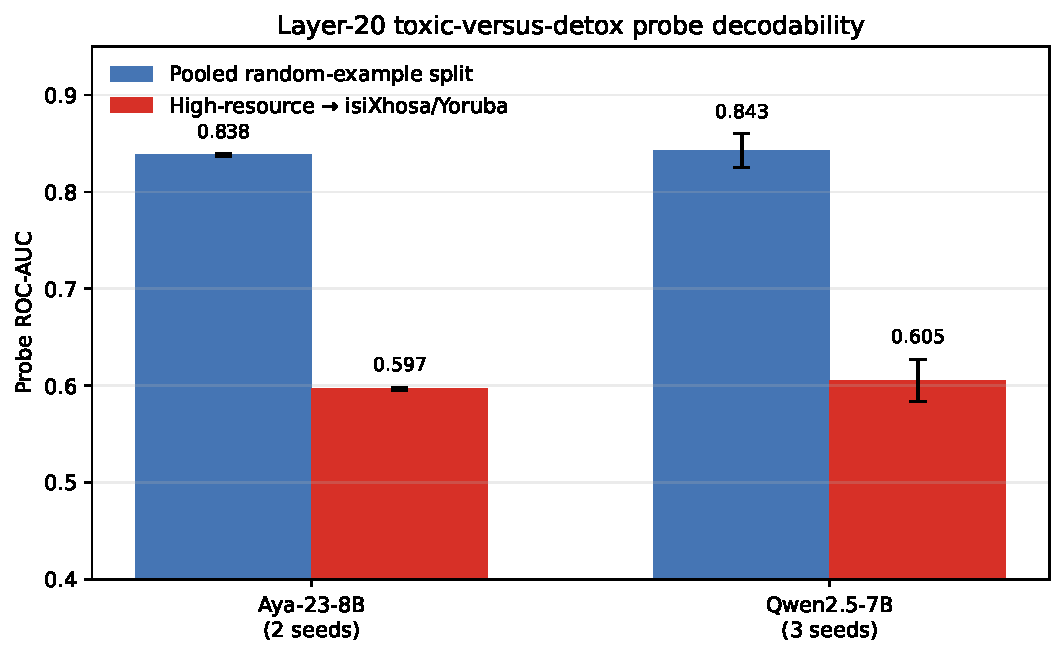
\includegraphics[width=\linewidth]{figures/fig_probe_decodability_transfer.pdf}
    \caption{Layer-20 representation decodability and higher-resource-to-lower-resource
    transfer. Bars show mean ROC-AUC across fine-tuning seeds; error bars are sample
    standard deviations. The transfer condition trains on Amharic, Arabic, German,
    English, Spanish, Hindi, and Ukrainian and evaluates on isiXhosa and Yoruba.}
    \label{fig:probe-transfer}
\end{figure}

\subsection{Qwen layer profile}

Qwen provides a three-seed profile at layers 10, 15, and 20. Pooled
random-example AUC generally increases toward later layers. Transfer is lower at every
stored layer, but layer 20 has the strongest transfer AUC in all three seeds:
0.5975, 0.6302, and 0.5884. Layer 20 is not the pooled-AUC optimum in every seed;
for seed 1337, layer 15 slightly exceeds layer 20. We therefore describe layer 20 as
the most consistently strong transfer layer rather than as universally optimal.

\begin{figure}[t]
    \centering
    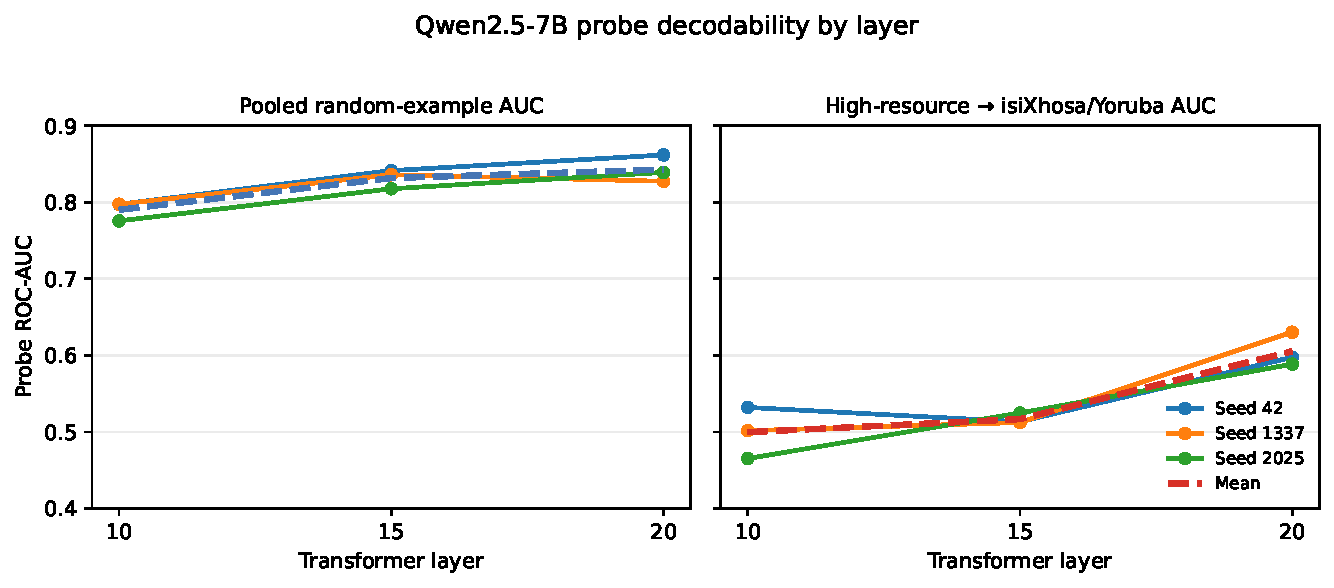
\includegraphics[width=\linewidth]{figures/fig_qwen_probe_layer_profile.pdf}
    \caption{Qwen2.5-7B probe decodability across layers. Solid lines show
    individual fine-tuning seeds; dashed lines show their mean. The right panel is the
    higher-resource-to-isiXhosa/Yoruba transfer condition.}
    \label{fig:qwen-layer-profile}
\end{figure}

\subsection{Candidate SAE features}

The recovered SAE analyses provide seed-specific candidate feature inventories.
For Aya seed 42, an 8,192-dimensional SAE is trained on 4,000 layer-20 activations
from 2,000 toxic/detox pairs. Qwen has corresponding summaries across three seeds.
These lists motivate candidate directions but do not by themselves establish semantic
interpretability, cross-seed alignment, or causal feature effects. Full inventories and
configuration details appear in the appendix.
